\documentclass[conference,a4paper]{IEEEtran}
\IEEEoverridecommandlockouts

\usepackage[T1]{fontenc}
\usepackage{amsmath,amssymb,amsfonts}
\usepackage{graphicx}
\graphicspath{{figures/}}
\usepackage{booktabs}
\usepackage{array}
\usepackage{tabularx}
\usepackage{xcolor}
\usepackage{tikz}
\usetikzlibrary{arrows.meta,positioning,calc}
\usepackage{xurl}
\usepackage[hidelinks]{hyperref}
\usepackage{cite}

\definecolor{binusblue}{HTML}{1F3A68}
\definecolor{rightgrid}{HTML}{E6F4EA}
\definecolor{leftgrid}{HTML}{E8F0FA}
\definecolor{ledger}{HTML}{FFF4E0}

\newcommand{\Mgha}{\,Mg\,ha$^{-1}$}

\begin{document}

\title{Can Satellites Replace the Field Plot? A Blind Benchmark of Satellite Forest Carbon and Conformal Crediting with Calibrated Risk}

\author{
\IEEEauthorblockN{Kenny Tang}
\IEEEauthorblockA{\textit{Computer Science Department}\\
\textit{Bina Nusantara University}\\
Jakarta, Indonesia 11480\\
kenny.tang@binus.ac.id}
\and
\IEEEauthorblockN{Riki Awal Syahputra}
\IEEEauthorblockA{\textit{Computer Science Department}\\
\textit{Bina Nusantara University}\\
Jakarta, Indonesia 11480\\
riki.syahputra@binus.ac.id}
\and
\IEEEauthorblockN{Richard Hans}
\IEEEauthorblockA{\textit{Computer Science Department}\\
\textit{Bina Nusantara University}\\
Jakarta, Indonesia 11480\\
richard.hans001@binus.ac.id}
\linebreakand
\IEEEauthorblockN{Evelyn Jane Sutjiadi}
\IEEEauthorblockA{\textit{Computer Science Department}\\
\textit{Bina Nusantara University}\\
Jakarta, Indonesia 11480\\
evelyn.sutjiadi@binus.ac.id}
\and
\IEEEauthorblockN{Yenny Chen}
\IEEEauthorblockA{\textit{Computer Science Department}\\
\textit{Bina Nusantara University}\\
Jakarta, Indonesia 11480\\
yenny.chen@binus.edu}
\and
\IEEEauthorblockN{Jude Joseph Lamug Martinez}
\IEEEauthorblockA{\textit{Computer Science Department}\\
\textit{Bina Nusantara University}\\
Jakarta, Indonesia 11480\\
jmartinez@binus.edu}
}
\makeatletter
\newcommand{\linebreakand}{%
  \end{@IEEEauthorhalign}
  \hfill\mbox{}\par
  \mbox{}\hfill
  \begin{@IEEEauthorhalign}
}
\makeatother
\maketitle

\begin{abstract}
Satellite platforms promise to replace field inventories in forest carbon crediting, but their estimates are rarely tested blind against the standard-formula answer, and credits are issued with deductions of unknown risk. We separate the question into two isolated grids. The right grid computes field ground truth to SNI 7724, IPCC, CDM, and Verra rules with a Monte Carlo uncertainty budget and is sealed. The left grid sees only plot coordinates and dates and estimates carbon from time-matched Sentinel-1/2, Landsat, PALSAR, canopy height, and GEDI lidar. A hash-chained commit-reveal ledger makes changes after the reveal detectable. On 476 plots, blind error was 21\% on 1\,ha plots and 7--9\% on project totals outside Indonesia, but near 100\% on small Indonesian plots. Only 21.5\% of Sentinel-2 acquisitions see an Indonesian plot clear, and a common scene filter discards 65\% of those; missing-data-augmented conformal regression kept 90\% intervals under full cloud. We propose conformal crediting, a lower bound calibrated on other projects with field truth. It met a 10\% over-crediting target for five maps within 2.9 points, was invariant to map inflation, and credited 72--84\% of the true stock without a field plot, while the VM0047 deduction over-credited 23--29\% of projects that had field plots. No satellite estimate of annual growth beat assuming no change.
\end{abstract}

\begin{IEEEkeywords}
forest carbon, MRV, remote sensing, cloud cover, conformal prediction, spatial cross-validation, carbon crediting, commit-reveal ledger, distributed processing
\end{IEEEkeywords}

%=====================================================================
\section{Introduction}
A forest carbon credit is issued on a number computed by a fixed chain. Field crews measure each stem's diameter $D$ and height $H$ and identify its species for wood density $\rho$; a pantropical allometric equation converts these to aboveground biomass (AGB)~\cite{chave2014improved}, and fixed factors convert AGB to carbon and CO$_2$~\cite{verra2025vm0047,ipcc2019v4}. The chain is the standard. What is costly is the field visit, above all in remote Indonesian forests. Satellite platforms, including our own NusaCarbon prototype, promise to replace the visit, and global biomass maps exist~\cite{santoro2021global,chloris2022}. Investigations of REDD+ crediting, however, show that unverifiable estimates produce over-crediting~\cite{west2023redd}.

How close is a satellite number to what the standard formula gives at the same place and time? Three traps inflate reported accuracy: \emph{leakage}, when a model is trained or tuned on plots next to those it is scored on~\cite{ploton2020spatial}; \emph{temporal mismatch} between the field and image dates; and \emph{scale}, when 0.05\,ha plots are compared with 10\,m to 4.6\,km pixels. An audit of our own platform found more: forest figures driven by default constants, clouds screened only at scene level, and a ``confidence'' grade computed from image metadata, none of it checked against field data.

We separate the problem into two grids (Fig.~\ref{fig:grids}). The \textbf{right grid} is fixed: public field plots, the standard formula, a carbon density. The \textbf{left grid} is free, any satellite data and any algorithm, subject to one rule: it never sees the right grid's outcomes for the plots it is scored on. We ask: \textbf{RQ1} (methodology) how far a blind satellite estimate deviates from standard-formula ground truth, by plot size and aggregation; \textbf{RQ2} (AI) which inputs and learners close the gap; \textbf{RQ3} how often clouds hide an Indonesian plot, and whether uncertainty can be stated honestly at plot and project scale; \textbf{RQ4} whether a credit can be issued at a stated, verified risk of over-crediting, and whether growth can be estimated; and \textbf{RQ5} (distributed systems) whether extraction can be sharded and made fault tolerant with bit-identical output.

\textbf{Contributions.} (i) A blind, time-matched protocol with a commit-reveal ledger, applied to 476 stock plots and 196 repeat-census plots. (ii) A right grid built to SNI 7724, IPCC, CDM, Verra, and Gold Standard rules with a Monte Carlo uncertainty budget. (iii) A plot-level Sentinel-2 clear-sky climatology for Indonesia and a measured error rate of the scene-level cloud filter. (iv) A test of missing-data-augmented conformal intervals under cloud with out-of-region calibration. (v) \emph{Conformal crediting}, a crediting rule with a calibrated over-crediting risk that is invariant to map inflation. (vi) A sharded, idempotent extraction runner. We propose no new estimator or interval method; conformal crediting reuses standard conformal machinery~\cite{lei2018distribution} for a new decision.

\begin{figure}[t]
\centering
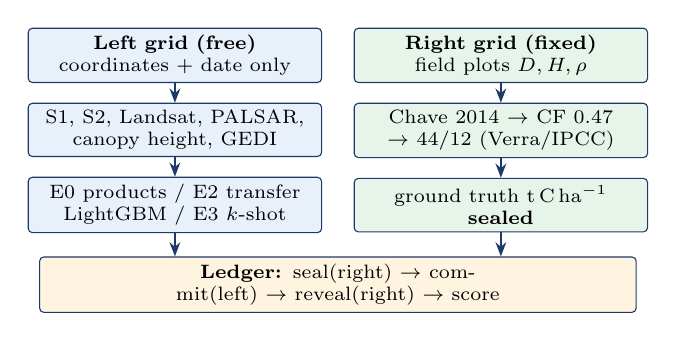
\begin{tikzpicture}[
  font=\scriptsize,
  box/.style={draw=binusblue,rounded corners=1.5pt,align=center,inner sep=2.5pt,text width=3.55cm},
  arr/.style={-{Stealth[length=1.8mm]},thick,binusblue}]
\node[box,fill=leftgrid] (L1) {\textbf{Left grid (free)}\\coordinates + date only};
\node[box,fill=leftgrid,below=2.5mm of L1] (L2) {S1, S2, Landsat, PALSAR,\\canopy height, GEDI};
\node[box,fill=leftgrid,below=2.5mm of L2] (L3) {E0 products / E2 transfer\\LightGBM / E3 $k$-shot};
\node[box,fill=rightgrid,right=4mm of L1] (R1) {\textbf{Right grid (fixed)}\\field plots $D,H,\rho$};
\node[box,fill=rightgrid,below=2.5mm of R1] (R2) {Chave 2014 $\to$ CF 0.47\\$\to$ 44/12 (Verra/IPCC)};
\node[box,fill=rightgrid,below=2.5mm of R2] (R3) {ground truth t\,C\,ha$^{-1}$\\\textbf{sealed}};
\node[box,fill=ledger,below=3mm of $(L3.south)!0.5!(R3.south)$,text width=7.4cm] (G) {\textbf{Ledger:} seal(right) $\rightarrow$ commit(left) $\rightarrow$ reveal(right) $\rightarrow$ score};
\draw[arr] (L1)--(L2); \draw[arr] (L2)--(L3); \draw[arr] (R1)--(R2); \draw[arr] (R2)--(R3);
\draw[arr] (L3.south)--(L3.south|-G.north); \draw[arr] (R3.south)--(R3.south|-G.north);
\end{tikzpicture}
\caption{Blind two-grid design. Only the manifest (plot id, coordinates, date, radius) crosses from right to left.}
\label{fig:grids}
\end{figure}

%=====================================================================
\section{Related Work}
\textbf{Standards.} The BIOMASS package propagates the uncertainty of Chave's allometry~\cite{rejou2017biomass}, and the frameworks of Table~\ref{tab:standards} prescribe plots, pools, and uncertainty rules.

\textbf{Remote sensing.} Optical and radar signals saturate over dense canopy. GEDI lidar samples canopy height in 25\,m footprints~\cite{duncanson2022gedi}; global maps include ESA CCI Biomass~\cite{santoro2021global}, Chloris~\cite{chloris2022}, and 1\,m and 10\,m canopy height~\cite{tolan2024meta,lang2023eth}. Sentinel-1 and PALSAR reached 31--38\% in Kalimantan against a lidar layer~\cite{berninger2018sar}, and airborne lidar 13\% at 1\,ha in Sabah~\cite{jucker2018estimating}. Southeast Asia is cloudy on at least 80\% of days~\cite{wilson2016cloud}.

\textbf{Validation and uncertainty.} Spatially blocked validation reveals far lower map skill than random validation~\cite{ploton2020spatial}. Conformal prediction gives finite-sample intervals~\cite{lei2018distribution}; conformalized quantile regression (CQR) adapts their width~\cite{romano2019cqr}, and Zaffran \textit{et al.} extend conformal prediction to missing covariates~\cite{zaffran2023conformal}. Map error must be separated from plot error~\cite{araza2022comprehensive}, and model-based variance estimators under-cover when spatial correlation is ignored~\cite{breidenbach2016empirical}. Conservative crediting asks that a credited stock exceed the truth with small probability~\cite{grassi2008applying}, which Neeff solves parametrically~\cite{neeff2021risk}.

%=====================================================================
\section{Methodology}

\subsection{Right Grid: Ground Truth by the Standards}
\textbf{Data.} The stock benchmark has 476 plots in 27 region blocks: 148 HCSA plots in six Indonesian provinces, nested 0.01/0.05\,ha~\cite{hcsa2023data}; 142 GEO-TREES network plots, pantropical~\cite{geotrees2024}; and 186 Labri\`ere 1\,ha units in French Guiana and Gabon~\cite{labriere2018insitu}. For change, the SAFE census in Sabah gives 25$\times$25\,m plots measured stem by stem with day-precision dates from 2010 to 2020~\cite{svatek2025safe}. Table~\ref{tab:standards} lists the rules we follow.

\begin{table}[t]
\centering
\caption{Frameworks Applied to the Right Grid}
\label{tab:standards}
\footnotesize
\setlength{\tabcolsep}{2.5pt}
\begin{tabularx}{\columnwidth}{@{}l l l X@{}}
\toprule
\textbf{Framework} & \textbf{Conf.} & \textbf{Prec.} & \textbf{Uncertainty rule}\\
\midrule
SNI 7724~\cite{sni7724} & -- & $\le$20\% & nested plots, five pools, Tier 3\\
HCSA v2.0~\cite{rosoman2017hcsa} & 90\% & $\pm$10\% & 0.01/0.05\,ha nested circles\\
IPCC 2006/2019~\cite{ipcc2019v4} & 95\% & -- & Approach 1 or 2 (Monte Carlo)\\
CDM AR-TOOL14~\cite{artool14} & 90\% & $\pm$10\% & stepped discount; sampling only\\
Verra VM0047~\cite{verra2025vm0047} & 90\% & -- & deduct $U-10\%$; 0 if $U>100\%$\\
Gold Standard~\cite{gs2024ar} & 90\% & $\pm$20\% & deduct the excess over 20\%\\
\bottomrule
\end{tabularx}
\end{table}

\textbf{Tree, plot, and carbon.} A tree's AGB follows Chave~2014 Eq.~4~\cite{chave2014improved},
\begin{equation}
\mathrm{AGB}_i=0.0673\,(\rho_i D_i^2 H_i)^{0.976}\ \text{[kg]},\qquad \sigma_{\ln}=0.357,
\label{eq:chave4}
\end{equation}
with height from a local $\ln H$--$\ln D$ model where it was not measured and wood density from the Global Wood Density Database at species, genus, or family level~\cite{rejou2017biomass}. Tree biomass is expanded by the area in which a stem of its size is counted, and pools and carbon follow IPCC and SNI 7724:
\begin{equation}
\begin{aligned}
\mathrm{AGB}_j&=\sum_{i\in j}\frac{\mathrm{AGB}_i}{1000\,a(D_i)},\quad a(D)=\begin{cases}0.01,&5\le D<15\\0.05,&D\ge 15\end{cases}\\
C_j&=\mathrm{CF}\,(1+R)\,\mathrm{AGB}_j,\qquad \mathrm{CO_2e}_j=\tfrac{44}{12}\,C_j,
\end{aligned}
\label{eq:plot}
\end{equation}
with CF $=0.47$ and root-to-shoot $R=0.37$ (SNI 7724, IPCC 2006) or 0.21 (IPCC 2019). The benchmark compares AGB, so CF and $R$ cancel and every relative error holds for t\,C\,ha$^{-1}$ and t\,CO$_2$e\,ha$^{-1}$. HCSA was recomputed tree by tree; whole plots with a missing input or an implausible stem were excluded, never imputed. One \textit{Gluta renghas} recorded at $D=480$\,cm, a circumference typed as a diameter, would have produced 4{,}426\Mgha. Palms are excluded because Eq.~\ref{eq:chave4} is for dicotyledonous trees.

\textbf{Uncertainty and deduction.} Plots are grouped into strata $h$ with weights $w_h$, and the project uncertainty at 90\% is $u=t_{0.95}\sqrt{\sum_h w_h^2s_h^2/n_h}/\bar b$ (AR-TOOL14)~\cite{artool14}. AR-TOOL14 counts sampling error only, so we add IPCC Approach~2: 2{,}000 Monte Carlo draws per tree of diameter, height, wood density, allometric residual, and CF errors with the BIOMASS error models~\cite{rejou2017biomass}. For change on the same plots, VM0047 v1.1 Eq.~28 gives
\begin{equation}
U=T\sqrt{SE_0^2+SE_1^2-2\rho\,SE_0SE_1}\,/\,\Delta C,
\label{eq:vm0047}
\end{equation}
where $\rho$ is the correlation of the two stock means; credits are multiplied by $1-\min(1,\max(0,U-0.1))$~\cite{verra2025vm0047}. The sealed outcome file never leaves the right grid; only the manifest does.

\subsection{Left Grid: Inputs and Estimators}
For each plot, using only coordinates and the field date $t_j$, the left grid reads clear observations within $t_j\pm90$\,days: Sentinel-2 L2A bands and indices, Landsat 5--9, Sentinel-1 backscatter, the annual ALOS PALSAR mosaic, and elevation. Through Google Earth Engine it also reads the Meta 1\,m and ETH 10\,m canopy height maps~\cite{tolan2024meta,lang2023eth}, GEDI L4A biomass and L2A height within 1\,km~\cite{duncanson2022gedi}, ESA CCI Biomass~\cite{santoro2021global}, and Hansen forest loss~\cite{hansen2013high}. \textbf{E0} reads published products as they are. \textbf{E2} is LightGBM~\cite{ke2017lightgbm} on $\ln\mathrm{AGB}$, trained on all region blocks except the target and predicting it blind (leave-one-region-out, LORO), with smearing retransformation. \textbf{E3} recalibrates E2 by the ratio on $k$ random plots of the target block. We score relative RMSE (rRMSE), bias, $R^2$, and the error of the mean of $n$ plots, which approximates a project total. Uncertainty of every claim comes from a region-block bootstrap (2{,}000 draws) and five seeds.

\subsection{Clouds}
\textbf{Climatology.} For 97 locations, we read the Sentinel-2 scene classification of every acquisition from 2021 to 2023 in a 5$\times$5 window of 20\,m pixels around the plot (22{,}697 acquisitions). An acquisition is \emph{clear} if every pixel is clear. We test the scene filter of many Earth Engine pipelines, ours included (\texttt{CLOUDY\_PIXEL\_PERCENTAGE}~$<30$), against this plot condition. \textbf{Missing optical data.} For a share $q$ of target plots we remove the optical block and compare a naive model, modality dropout~\cite{neverova2016moddrop}, a cloud-aware switch to a radar model, and imputation of optical features from radar.

\subsection{Confidence: Plot and Project Intervals}
All intervals target 90\% and are calibrated on inner LORO residuals of the training regions only. CQR~\cite{romano2019cqr} scores $s=\max\{\hat q_{\mathrm{lo}}(x)-y,\,y-\hat q_{\mathrm{hi}}(x)\}$ on $y=\ln\mathrm{AGB}$ and widens the quantile band by the conformal quantile of $s$. \emph{Cloud-aware} CQR scores each calibration plot twice, as observed and with its optical block removed, and gives each test plot the threshold of its own missingness pattern, a two-pattern case of CP-MDA~\cite{zaffran2023conformal}. Its guarantee assumes missingness independent of the outcome, which clouds violate, so coverage must be measured. A project's satellite mean has errors that share one regional bias, so its standard error is
\begin{equation}
SE^2=s_w^2/n+s_b^2,
\label{eq:twocomp}
\end{equation}
with $s_w$ and $s_b$ the within- and between-region spread of log residuals in other regions. With $k$ field plots, the satellite becomes auxiliary data for a ratio estimator.

\subsection{Conformal Crediting}
A registry issues a number, not an interval. It should be a lower bound that exceeds the true stock in at most a share $\delta$ of projects~\cite{grassi2008applying,neeff2021risk}. For a satellite map no design-based standard error exists, so we calibrate the bound on other projects with field truth. Project $j$ has estimate $\hat Y_j$, true mean $Y_j$, and relative standard error $r_j$ ($r_j=1$ if none); its score is $z_j=\ln(\hat Y_j/Y_j)/r_j$. With scores from $m$ calibration projects, a new project is credited
\begin{equation}
C=\hat Y\exp(-q\,r),\qquad q=z_{(\lceil (m+1)(1-\delta)\rceil)}.
\label{eq:cc}
\end{equation}
If projects are exchangeable, $P(C>Y)\le\delta$, as in split conformal prediction with projects as units~\cite{lei2018distribution}; plots inside a project may be correlated in any way. The rule needs $m\ge1/\delta-1$ projects, nine for $\delta=0.1$. If every map value is multiplied by $c$, every plain score shifts by $\ln c$, so $q$ shifts by $\ln c$ and $C$ is unchanged: \emph{inflating a map earns no credit}. We split regions of 16 or more plots into spatial sub-projects of about 10 plots, giving 31 projects in 19 regions, and calibrate each project only on projects from other regions. We score the realised over-crediting rate and the \emph{yield}, the mean share $C_j/Y_j$ of the true stock credited.

\subsection{Ledger and Distributed Extraction}
Every protocol step is an entry in an append-only log carrying the SHA-256 of the previous entry~\cite{haber1991timestamp}: \texttt{seal} (digest of the sealed outcomes), \texttt{commit} (digest of each prediction file), \texttt{release} (training labels per fold, flagged if any target label is included), and \texttt{reveal}, accepted only if the sealed file still matches. Commits after a reveal are refused. An extraction task is one (plot, date, window, sensor) request, stored under the hash of the canonical task, which makes re-execution idempotent and the cache a checkpoint. Transient errors are retried with capped exponential backoff. Spatial tiles are split when they exceed the mean load and placed by consistent hashing~\cite{karger1997consistent} or the longest-processing-time (LPT) rule~\cite{graham1969bounds}.

%=====================================================================
\section{Results}

\subsection{How Certain Is the Right Grid?}
On the 148 HCSA plots, the Monte Carlo 95\% interval of plot AGB has a median half-width of 31\%. The standards' own choices are large. The SNI 7724 root-to-shoot ratio gives 13\% more carbon than the 2019 Refinement, and the regional equation of Basuki \textit{et al.} moves provincial stocks from $-40$\% to $+121$\% against Chave. By AR-TOOL14, the provincial sampling uncertainty is 9--34\%, but measurement and allometric error, which AR-TOOL14 ignores, carry 10--64\% of the variance of the mean. The same data receive deductions of 24\% under VM0047, 34\% under AR-TOOL14, and 14\% under Gold Standard (Jambi). Field truth is still far more precise than the satellite: the implied standard error of a Labri\`ere unit is 5\%. Growth is harder. With 9--16 plots of 0.06\,ha per SAFE block, Eq.~\ref{eq:vm0047} with $\rho=0$ deducts 100\% of the credit for 13 of 15 blocks. With the measured $\rho$ (0.45--0.99), seven blocks keep some credit.

\subsection{Blind Accuracy (RQ1) and Closing the Gap (RQ2)}
Table~\ref{tab:acc} gives the blind errors. The confirmatory E2, committed before the reveal, missed by 48.5\% overall, 28.6\% on the 1\,ha units, 41.9\% on GEO-TREES, and 102.9\% on HCSA, where neither committed estimator beat predicting the mean. Plot size dominates the error. The largest gain came from inputs, not algorithms: adding the 1\,m canopy height map and GEDI cut the overall error by 9.0 points (bootstrap 95\% interval $-13.0$ to $-6.1$), to 20.6\% on the 1\,ha units and 27.7\% on GEO-TREES, and raised $R^2$ from 0.29 to 0.53. Read as published, GEDI under-estimated by 29--41\%: lidar helps as an input, not as an answer.

\begin{table}[t]
\centering
\caption{Blind rRMSE (\%) Against the Right Grid, Leave-One-Region-Out}
\label{tab:acc}
\footnotesize
\setlength{\tabcolsep}{3pt}
\begin{tabular}{@{}l r r r r@{}}
\toprule
\textbf{Left-grid estimate} & \textbf{All} & \textbf{GEO-T.} & \textbf{HCSA} & \textbf{1\,ha}\\
\midrule
E0 Chloris, as published & 49.2 & 37.4 & 107.1 & 30.7\\
E0 ESA CCI, as published & 49.4 & 38.8 & 105.4 & 31.5\\
E0 GEDI L4A, as published & 59.2 & 50.0 & 107.0 & 46.6\\
E2 (S1/S2, Landsat, PALSAR, DEM) & 49.1 & 42.0 & 104.8 & 28.8\\
\quad + GEDI & 45.5 & 36.6 & 102.4 & 24.5\\
\quad + canopy height & 41.5 & 32.2 & \textbf{94.8} & 22.4\\
\quad + canopy height + GEDI & \textbf{40.1} & \textbf{27.7} & 95.6 & \textbf{20.6}\\
\midrule
Gain over E2 (points) & $-9.0$ & $-14.3$ & $-9.2$ & $-8.2$\\
\bottomrule
\end{tabular}

\vspace{2pt}
{\scriptsize 475 plots with AGB $>$1\Mgha: GEO-TREES 142, HCSA 148 (0.05\,ha), Labri\`ere 185 (1\,ha). Region-bootstrap 95\% intervals of the gain row all exclude zero.\par}
\end{table}

\textbf{Where the error comes from.} Predictions saturate (Fig.~\ref{fig:scatter}): above 400\Mgha{} (mean 480) the E2 mean is 293, and below 50 (mean 21) it is 60, while between 100 and 300\Mgha{} the median error is only $+5$ to $+12$\%. The HCSA plots hold a median of 15 stems, so one large tree moves a plot by hundreds of Mg\,ha$^{-1}$, which no 10--30\,m pixel can resolve. Narrowing the time window from 365 to 30 days changed the Indonesian error by under three points.

\begin{figure}[t]
\centering
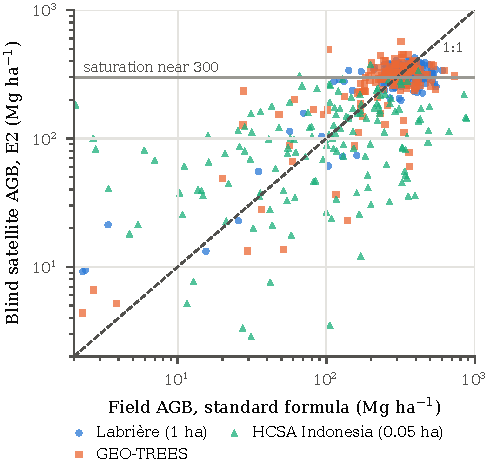
\includegraphics[width=0.84\columnwidth]{fig_scatter}
\caption{Blind E2 against the field value, 476 plots (log axes). Predictions flatten above about 300\Mgha; small HCSA plots scatter widely.}
\label{fig:scatter}
\end{figure}

\textbf{Aggregation and local plots.} Credits are issued for areas, not plots. With canopy height and GEDI and no field plot, the median error of a block total was 7\% on the 1\,ha units, 9\% on GEO-TREES, and 20\% on HCSA, and the mean of 20 plots was within 3--5\% of its field mean outside Indonesia. A ratio correction on $k=10$--20 local plots (E3) brought the original E2 block totals from 29\% to 9--10\% on GEO-TREES and from 11\% to 6\% on Labri\`ere. On HCSA it hurt until $k=20$, because a few small plots are a worse calibrator than none.

\textbf{Reliability.} Seed noise is small (SD 0.36 points), but region sampling is not: the overall E2 interval is 35--69\%. The dataset differences and the canopy height and GEDI gain survive it; E2 versus Chloris and radar versus optical do not.

\subsection{Clouds and Confidence (RQ3)}
\textbf{How often is a plot clear?} On a median Indonesian location, only 21.5\% of Sentinel-2 acquisitions see the plot fully clear (Sabah 26\%, Africa 17\%, the Americas 39\%), falling to 7.6\% in January and peaking at 33.5\% in May. Revisit compensates: the median gap between clear looks is 10 days, and 96\% of dates have one within $\pm$30 days. \emph{The scene filter is the real problem.} In Indonesia, \texttt{CLOUDY\_PIXEL\_PERCENTAGE}~$<30$ keeps 11.5\% of acquisitions, but 34\% of those are cloudy over the plot, and it throws away 65\% of the clear ones. Masking at the plot gives 2.8 times as many clear looks.

\textbf{What clouds cost.} Because the model leans on radar, terrain, and annual products, removing every optical feature raised the error only from 48.0\% to 50.0\%. Modality dropout and the switch handle partial cloud equally well. Imputing optical features from radar was harmful (bias $-61$\% at full cloud).

\begin{table}[t]
\centering
\caption{90\% Intervals, Leave-One-Region-Out: Coverage and Median Upper/Lower Ratio}
\label{tab:int}
\footnotesize
\setlength{\tabcolsep}{3.5pt}
\begin{tabular}{@{}l l r r r@{}}
\toprule
\textbf{Method} & \textbf{Optical data} & \textbf{All} & \textbf{HCSA} & \textbf{Ratio}\\
\midrule
Split conformal & as observed & 0.884 & 0.682 & 16.3\\
Normalized conformal & as observed & 0.794 & 0.723 & 3.3\\
CQR & as observed & \textbf{0.899} & \textbf{0.811} & 5.3\\
CQR & all removed & 0.865 & 0.70 & 5.4\\
Cloud-aware CQR & all removed & \textbf{0.905} & 0.77 & 7.8\\
\bottomrule
\end{tabular}
\end{table}

\textbf{Which intervals are honest?} Table~\ref{tab:int} compares interval methods. CQR is the only one that reaches the target with usable width (89.9\%, upper bound 5.3 times the lower); split conformal is three times wider, and normalized conformal under-covers because a difficulty model fitted on other regions does not transfer. When every target plot is clouded, plain CQR falls to 86.5\%, and cloud-aware CQR keeps 90.5\% by widening honestly ($+4.0$ points, interval $+1.9$ to $+6.6$). HCSA stays under-covered (68--81\%) by every method, a shift that marginal guarantees do not cover. A platform-style metadata confidence score, rebuilt from cloud cover, completeness, and temporal offset, carries no information about error once the dataset is controlled for (partial rank correlation $-0.03$ to $+0.07$).

\textbf{Projects.} For 19 projects (blocks with at least eight plots), a naive interval with independent plot errors covered only 74\% (HCSA 33\%). The two-component interval of Eq.~\ref{eq:twocomp} covered all 19, at a half-width of 71--86\%, which under VM0047 deducts most of the credit. With field plots, the satellite as auxiliary data made the ratio estimator 1.4--2.3 times as efficient as field plots alone on the large-plot datasets: the plots needed for $\pm$10\% fell from 408 to 216 (GEO-TREES) and from 381 to 162 (Labri\`ere). On HCSA it saved none.

\subsection{From Intervals to Credits and Growth (RQ4)}
Table~\ref{tab:cc} credits the 31 projects at $\delta=0.10$. Crediting the raw map over-credits 35\% of projects. VM0047 on the honest two-component uncertainty never over-credits but credits only 48\% of the true stock. Conformal crediting meets its target: 9.7\% of projects are over-credited, and 72\% of the true stock is credited without a field plot in the project, 84\% with the canopy height and GEDI map. A better map buys credits; it does not buy risk. With field plots, the VM0047 deduction still over-credits 23\% of projects with 5 plots and 29\% with 10 (yield 90\%), because the deduction only starts above 10\% uncertainty. The design lower bound at the same $\delta$ meets the target (8.5\% with 10 plots, yield 86\%), and studentized conformal calibration matches it.

\begin{table}[t]
\centering
\caption{Crediting Rules at $\delta=0.10$, 31 Projects, Cross-Region Calibration}
\label{tab:cc}
\footnotesize
\setlength{\tabcolsep}{4pt}
\begin{tabular}{@{}l r r@{}}
\toprule
\textbf{Rule} & \textbf{Over-credited} & \textbf{Yield}\\
\midrule
\multicolumn{3}{@{}l}{\emph{Satellite only (no plot in the project)}}\\
No deduction & 35.5\% & 94.4\%\\
VM0047, two-component $U$ & 0.0\% & 47.8\%\\
Parametric bound, independent errors & 9.7\% & 72.6\%\\
Conformal (Eq.~\ref{eq:cc}) & 9.7\% & 72.2\%\\
Conformal, canopy height + GEDI map & 9.7\% & 84\%\\
\midrule
\multicolumn{3}{@{}l}{\emph{Satellite + 5 random field plots (ratio estimator)}}\\
VM0047 ($U-10\%$) & 22.6\% & 82.2\%\\
Design lower bound & 9.9\% & 80.7\%\\
Conformal, studentized & 9.6\% & 80.7\%\\
\bottomrule
\end{tabular}
\end{table}

\textbf{Whatever the map?} Applied to five maps (E2, Chloris, their average, and E2 inflated by 10\% and 20\%), the conformal bound's realised over-crediting stayed within 2.9 points of the target, against 9.4 for the parametric bound. Under the parametric bound, a map inflated by 20\% earns 87\% of the true stock instead of 73\% and doubles the over-crediting rate; under conformal crediting it earns the same 72.2\%. Fig.~\ref{fig:frontier} shows that both VM0047 points lie below the integrity-yield frontier, and it prices a field plot: at about 10\% risk the satellite alone earns 72\% of the true stock, 5 plots 81\%, and 10 plots 86\%. The guarantee is only as good as the calibration bank: with six to eight projects of one type, the bound reached the largest score and yield fell to 18\%.

\begin{figure}[t]
\centering
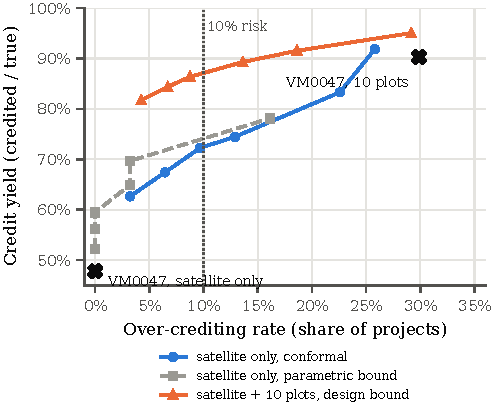
\includegraphics[width=0.84\columnwidth]{fig_frontier}
\caption{Integrity-yield frontier: realised over-crediting against yield as $\delta$ varies from 0.05 to 0.30. Crosses mark the VM0047 deduction.}
\label{fig:frontier}
\end{figure}

\textbf{Growth.} Chave's equation is invalid for palms (SAFE oil-palm plots came out at 505\Mgha), so a subset fixed before the reveal excludes them, leaving 196 plots with a mean gain of 1.87\Mgha\,yr$^{-1}$. At plot level, the Chloris difference had the same error as predicting no change (RMSE 8.06 vs 8.12), and the E2 stock difference was twice as bad with the wrong sign, because Sentinel-1 existed at the second census but not the first. A plot-scale stock error of 30--100\% cannot resolve growth of 1\% per year. The plain mean rate of the other blocks was the most accurate estimator (block MAE 0.98 vs 2.05 for no change), and adding PALSAR 2010, CCI change, and Hansen loss did not beat it (1.20).

\subsection{Systems (RQ5)}
The stock extraction ran 2{,}052 tasks on 24 workers in 2.1\,h. Splitting dense tiles cut the worst-worker load factor from 6.75 to 1.40 (LPT; measured 1.47); retries absorbed 85 transient errors, and 17 tasks (0.8\%) hit unreadable files. Throughput rose 5.1-fold up to 8 workers, then flattened at the slowest remote read. Results were bit-identical to the single-worker run at every worker count, under injected faults, and after a resume from the cache. The 37-entry ledger verifies end to end, and no fold released a label from its target block.

%=====================================================================
\section{Discussion}
\textbf{Can satellites replace the field plot?} Not at plot scale, and not for growth. Tested blind, open satellite data put a 1\,ha plot's stock within about 21\%, against 13\% for airborne lidar in Sabah~\cite{jucker2018estimating} and 31--38\% reported for radar in Kalimantan against a lidar layer~\cite{berninger2018sar}, but a 0.05\,ha plot within about 100\%. For growth, the quantity credits are paid on, no satellite estimator beat a regional average of measured growth. What satellites do well is \emph{replace part of the inventory}: project totals within 7--9\% outside Indonesia, and half the field plots where plots are large enough to rank.

\textbf{The ground truth is a model too.} Two valid standards differ by 13\% in total carbon, and deductions for the same data range from 14 to 34\%. ``100\% accuracy'' has no meaning; the meaningful target is to fall within the fully computed uncertainty of a field estimate made to a stated standard.

\textbf{Confidence must be calibrated, not graded.} A metadata score said nothing about error, and the $U-10\%$ deduction is not a lower confidence bound. Conformal crediting makes the over-crediting rate a design parameter and removes the reward for inflating the map. Its novelty is narrow: the target is that of Grassi and Neeff, the machinery is split conformal prediction, and conformal bounds for area-level parameters exist elsewhere~\cite{zhang2026conformal}; we have not found a crediting rule calibrated across projects against field truth and tested under transfer and biased maps.

\textbf{Implications and roadmap.} For NusaCarbon the evidence implies per-pixel cloud masking at the plot, a radar-led model with canopy height and GEDI, a cloud-aware CQR interval instead of a letter grade, conformal crediting from a bank of at least nine field-verified projects, and growth from remeasured permanent plots. Fine canopy structure gave the largest gain, which motivates the planned drone tiers: a DJI Matrice 350 RTK with a Zenmuse L2 lidar above the canopy, and an under-canopy swarm to measure stem diameters, where piloted under-canopy scanning has reached 0.6--0.9\,cm DBH error~\cite{hyyppa2020under}. Swarm-measured plots then become the sealed right grid, and three hypotheses are to be tested on Indonesian 1\,ha plots: swarm DBH within 3\% of tape, lidar AGB within 15\%, and repeat-flight growth beating the regional default rate.

\textbf{Threats to validity.} Only E0, E2, and the first change estimates are confirmatory; all later experiments were defined after the reveal and are exploratory, and we report every variant we ran. GEDI and Chloris were calibrated on field data that may include some of our sites. HCSA and Labri\`ere dates are known only to the year. Projects are region blocks, not registered projects.

%=====================================================================
\section{Conclusion}
We tested blind, against a sealed standard-formula right grid, whether open satellite data can replace the field plot. Satellites reached 21\% error on 1\,ha plots and 7--9\% on project totals, but failed on small plots and growth. Plot-level cloud masking nearly triples usable optical data, cloud-aware CQR keeps intervals honest, and conformal crediting issues credits at a stated risk without a field plot, unaffected by map inflation.

\section*{Data and Code Availability}
Field data are public~\cite{hcsa2023data,geotrees2024,labriere2018insitu,svatek2025safe}. Code, results, an extended version with all tables, and an interactive dashboard are at \url{https://github.com/kennytangg/carbon-paper}.

\begin{thebibliography}{37}

\bibitem{chave2014improved}
J. Chave \textit{et al.}, ``Improved allometric models to estimate the aboveground biomass of tropical trees,'' \textit{Global Change Biol.}, vol. 20, no. 10, pp. 3177--3190, 2014, doi: 10.1111/gcb.12629.

\bibitem{verra2025vm0047}
Verra, \textit{VM0047 Afforestation, Reforestation, and Revegetation}, ver. 1.1, May 2025. [Online]. Available: \url{https://verra.org/wp-content/uploads/2025/05/VM0047-v1.1_Final.pdf}

\bibitem{ipcc2019v4}
IPCC, \textit{2019 Refinement to the 2006 IPCC Guidelines for National Greenhouse Gas Inventories, Vol.~4}, Ch.~4 Forest Land, Table~4.4 (Updated). Geneva: IPCC, 2019.

\bibitem{santoro2021global}
M. Santoro \textit{et al.}, ``The global forest above-ground biomass pool for 2010 estimated from high-resolution satellite observations,'' \textit{Earth Syst. Sci. Data}, vol. 13, pp. 3927--3950, 2021.

\bibitem{chloris2022}
Chloris Geospatial, ``Global aboveground biomass stock and change, 2003--2019,'' distributed by the Microsoft Planetary Computer. [Online]. Available: \url{https://planetarycomputer.microsoft.com/dataset/chloris-biomass}

\bibitem{west2023redd}
T. A. P. West \textit{et al.}, ``Action needed to make carbon offsets from forest conservation work for climate change mitigation,'' \textit{Science}, vol. 381, no. 6660, pp. 873--877, 2023.

\bibitem{ploton2020spatial}
P. Ploton \textit{et al.}, ``Spatial validation reveals poor predictive performance of large-scale ecological mapping models,'' \textit{Nat. Commun.}, vol. 11, Art. no. 4540, 2020.

\bibitem{lei2018distribution}
J.~Lei, M.~G'Sell, A.~Rinaldo, R.~J. Tibshirani, and L.~Wasserman, ``Distribution-free predictive inference for regression,'' \textit{J. Amer. Statist. Assoc.}, vol.~113, no.~523, pp.~1094--1111, 2018, doi: 10.1080/01621459.2017.1307116.

\bibitem{rejou2017biomass}
M. R\'ejou-M\'echain, A. Tanguy, C. Piponiot, J. Chave, and B. H\'erault, ``BIOMASS: An R package for estimating above-ground biomass and its uncertainty in tropical forests,'' \textit{Methods Ecol. Evol.}, vol. 8, no. 9, pp. 1163--1167, 2017.

\bibitem{duncanson2022gedi}
L. Duncanson \textit{et al.}, ``Aboveground biomass density models for NASA's Global Ecosystem Dynamics Investigation (GEDI) lidar mission,'' \textit{Remote Sens. Environ.}, vol. 270, Art. no. 112845, 2022.

\bibitem{tolan2024meta}
J.~Tolan \textit{et al.}, ``Very high resolution canopy height maps from RGB imagery using self-supervised vision transformer and convolutional decoder trained on aerial lidar,'' \textit{Remote Sens. Environ.}, vol.~300, art.~113888, 2024, doi: 10.1016/j.rse.2023.113888.

\bibitem{lang2023eth}
N.~Lang, W.~Jetz, K.~Schindler, and J.~D. Wegner, ``A high-resolution canopy height model of the Earth,'' \textit{Nature Ecol. Evol.}, vol.~7, pp.~1778--1789, 2023, doi: 10.1038/s41559-023-02206-6.

\bibitem{berninger2018sar}
A.~Berninger, S.~Lohberger, M.~St\"angel, and F.~Siegert, ``SAR-based estimation of above-ground biomass and its changes in tropical forests of Kalimantan using L- and C-band,'' \textit{Remote Sens.}, vol.~10, no.~6, art.~831, 2018, doi: 10.3390/rs10060831.

\bibitem{jucker2018estimating}
T.~Jucker \textit{et al.}, ``Estimating aboveground carbon density and its uncertainty in Borneo's structurally complex tropical forests using airborne laser scanning,'' \textit{Biogeosciences}, vol.~15, pp.~3811--3830, 2018, doi: 10.5194/bg-15-3811-2018.

\bibitem{wilson2016cloud}
A.~M. Wilson and W.~Jetz, ``Remotely sensed high-resolution global cloud dynamics for predicting ecosystem and biodiversity distributions,'' \textit{PLoS Biol.}, vol.~14, no.~3, e1002415, 2016, doi: 10.1371/journal.pbio.1002415.

\bibitem{romano2019cqr}
Y.~Romano, E.~Patterson, and E.~Cand\`es, ``Conformalized quantile regression,'' in \textit{Adv. Neural Inf. Process. Syst. 32}, 2019, pp.~3543--3553.

\bibitem{zaffran2023conformal}
M.~Zaffran, A.~Dieuleveut, J.~Josse, and Y.~Romano, ``Conformal prediction with missing values,'' in \textit{Proc. 40th Int. Conf. Machine Learning (ICML)}, PMLR vol.~202, 2023, pp.~40578--40604.

\bibitem{araza2022comprehensive}
A.~Araza \textit{et al.}, ``A comprehensive framework for assessing the accuracy and uncertainty of global above-ground biomass maps,'' \textit{Remote Sens. Environ.}, vol.~272, art.~112917, 2022, doi: 10.1016/j.rse.2022.112917.

\bibitem{breidenbach2016empirical}
J.~Breidenbach, R.~E. McRoberts, and R.~Astrup, ``Empirical coverage of model-based variance estimators for remote sensing assisted estimation of stand-level timber volume,'' \textit{Remote Sens. Environ.}, vol.~173, pp.~274--281, 2016, doi: 10.1016/j.rse.2015.07.026.

\bibitem{grassi2008applying}
G.~Grassi \textit{et al.}, ``Applying the conservativeness principle to REDD to deal with the uncertainties of the estimates,'' \textit{Environ. Res. Lett.}, vol.~3, art.~035005, 2008, doi: 10.1088/1748-9326/3/3/035005.

\bibitem{neeff2021risk}
T.~Neeff, ``What is the risk of overestimating emission reductions from forests -- and what can be done about it?'' \textit{Climatic Change}, vol.~166, art.~26, 2021, doi: 10.1007/s10584-021-03079-z.

\bibitem{hcsa2023data}
High Carbon Stock Approach, ``Forest field plot data for indicative HCS mapping, Indonesia,'' Fair Forward/GIZ and JKPP, 2023, CC BY-SA 4.0. [Online]. Available: \url{https://huggingface.co/datasets/fair-forward/hcsa_indonesia}

\bibitem{geotrees2024}
GEO-TREES, ``Biomass reference plot data,'' IIASA, accessed Oct. 2026. [Online]. Available: \url{https://geo-trees.nodes.iiasa.ac.at/page/data}

\bibitem{labriere2018insitu}
N. Labri\`ere \textit{et al.}, ``In situ reference datasets from the TropiSAR and AfriSAR campaigns in support of upcoming spaceborne biomass missions,'' \textit{IEEE J. Sel. Topics Appl. Earth Observ. Remote Sens.}, vol. 11, no. 10, pp. 3617--3627, 2018, doi: 10.1109/JSTARS.2018.2851606.

\bibitem{svatek2025safe}
M. Sv\'atek \textit{et al.}, ``Tree census data from the SAFE Project 2011--2020,'' Zenodo, 2025, doi: 10.5281/zenodo.14882506.

\bibitem{sni7724}
Badan Standardisasi Nasional, \textit{SNI 7724:2011 Pengukuran dan penghitungan cadangan karbon -- Pengukuran lapangan untuk penaksiran cadangan karbon hutan (ground based forest carbon accounting)}. Jakarta: BSN, 2011.

\bibitem{rosoman2017hcsa}
G. Rosoman, S. S. Sheun, C. Opal, P. Anderson, and R. Trapshah, Eds., \textit{The HCS Approach Toolkit}, ver. 2.0, Module 4. Singapore: HCS Approach Steering Group, 2017.

\bibitem{artool14}
UNFCCC CDM Executive Board, \textit{A/R Methodological Tool 14: Estimation of Carbon Stocks and Change in Carbon Stocks of Trees and Shrubs in A/R CDM Project Activities}, ver.~04.2.

\bibitem{gs2024ar}
Gold Standard, \textit{Afforestation/Reforestation GHG Emissions Reduction \& Sequestration Methodology}, ver.~2.1, May 2024.

\bibitem{hansen2013high}
M.~C. Hansen \textit{et al.}, ``High-resolution global maps of 21st-century forest cover change,'' \textit{Science}, vol.~342, pp.~850--853, 2013, doi: 10.1126/science.1244693.

\bibitem{ke2017lightgbm}
G. Ke \textit{et al.}, ``LightGBM: A highly efficient gradient boosting decision tree,'' in \textit{Adv. Neural Inf. Process. Syst. 30}, 2017, pp. 3146--3154.

\bibitem{neverova2016moddrop}
N.~Neverova, C.~Wolf, G.~Taylor, and F.~Nebout, ``ModDrop: Adaptive multi-modal gesture recognition,'' \textit{IEEE Trans. Pattern Anal. Mach. Intell.}, 2016, doi: 10.1109/TPAMI.2015.2461544.

\bibitem{haber1991timestamp}
S. Haber and W. S. Stornetta, ``How to time-stamp a digital document,'' \textit{J. Cryptology}, vol. 3, no. 2, pp. 99--111, 1991.

\bibitem{karger1997consistent}
D. Karger, E. Lehman, T. Leighton, R. Panigrahy, M. Levine, and D. Lewin, ``Consistent hashing and random trees,'' in \textit{Proc. 29th ACM Symp. Theory Comput.}, 1997, pp. 654--663.

\bibitem{graham1969bounds}
R. L. Graham, ``Bounds on multiprocessing timing anomalies,'' \textit{SIAM J. Appl. Math.}, vol. 17, no. 2, pp. 416--429, 1969.

\bibitem{zhang2026conformal}
L.-C. Zhang and T.~Tuoto, ``Conformal confidence intervals with an application to small area estimation,'' arXiv:2608.02766, 2026.

\bibitem{hyyppa2020under}
E.~Hyypp\"a \textit{et al.}, ``Under-canopy UAV laser scanning for accurate forest field measurements,'' \textit{ISPRS J. Photogramm. Remote Sens.}, vol.~164, pp.~41--60, 2020, doi: 10.1016/j.isprsjprs.2020.03.021.

\end{thebibliography}

\end{document}
